\documentclass[12pt]{article}

%\usepackage{tjlreport}

% For graphical models:
\usepackage{tikz}
\usetikzlibrary{bayesnet}


%+++++++++++++++++++++++++++++++++++++++++++++++++++++++++++++++++++++++++++++++
\begin{document}
%+++++++++++++++++++++++++++++++++++++++++++++++++++++++++++++++++++++++++++++++

\title{Simple DAG demo\\ using TikZ and tikz-bayesnet}
\maketitle


\begin{figure}[ht]
\centering
\resizebox{.125\textheight}{!}{%  <--- comment out the return
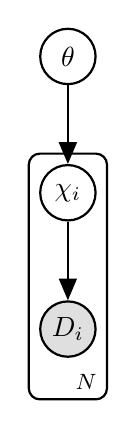
\begin{tikzpicture}[thick]

  % Nodes:
  \node[obs] (data) {$D_i$};
  \node[latent, above=of data] (char) {$\chi_i$};
  \node[latent, above=of char] (popn) {$\theta$};

  % Connections:
  \edge {popn} {char} ; %
  \edge {char} {data} ; %

  % Plate:
  \plate {source} {(char)(data)} {$N$} ;

\end{tikzpicture}%  <--- comment out the return @ end of resizebox
}
\caption{DAG for a simple two-level hierarchical model.}
\end{figure}


%+++++++++++++++++++++++++++++++++++++++++++++++++++++++++++++++++++++++++++++++
\end{document}
%+++++++++++++++++++++++++++++++++++++++++++++++++++++++++++++++++++++++++++++++
